\documentclass[aspectratio=43,english]{beamer} %If you want to create Polish presentation, replace 'english' with 'polish' and uncomment 3-th line, i.e., '\usepackage{polski}'
\usepackage[utf8]{inputenc}
\usepackage{polski} %Uncomment for Polish language
\usepackage{babel}
\usepackage{listings} %We want to put listings

\mode<beamer>{ 	%in 'beamer' mode
	\hypersetup{pdfpagemode=FullScreen}		%Enable Full screen mode
	\usetheme{JuanLesPins} 		%Show part title in right footer
	%\usetheme[dark]{AGH}                 		%Use dark background
	%\usetheme[dark,parttitle=leftfooter]{AGH}  	%Use dark background and show part title in left footer
}
\mode<handout>{	%in 'handout' mode
	\hypersetup{pdfpagemode=None}		
	\usepackage{pgfpages}
  	\pgfpagesuselayout{4 on 1}[a4paper,border shrink=5mm,landscape]	%show 4 slides on 1 page
  	\usetheme{boxes}
  	\addheadbox{structure}{\quad\insertpart\hfill\insertsection\hfill\insertsubsection\qquad} 	%content of header
 	\addfootbox{structure}{\quad\insertauthor\hfill\insertframenumber\hfill\insertsubtitle\qquad} 	%content of footer
}

\AtBeginPart{ %At begin part: display its name
	\frame{\partpage}
} 


%%%%%%%%%%% Configuration of the listings package %%%%%%%%%%%%%%%%%%%%%%%%%%
% Source: https://en.wikibooks.org/wiki/LaTeX/Source_Code_Listings#Using_the_listings_package
%%%%%%%%%%%%%%%%%%%%%%%%%%%%%%%%%%%%%%%%%%%%%%%%%%%%%%%%%%%%%%%%%%%%%%%%%%%%
\lstset{ %
  backgroundcolor=\color{white},   % choose the background color
  basicstyle=\footnotesize,        % the size of the fonts that are used for the code
  breakatwhitespace=false,         % sets if automatic breaks should only happen at whitespace
  breaklines=true,                 % sets automatic line breaking
  captionpos=b,                    % sets the caption-position to bottom
  commentstyle=\color{green},      % comment style
  deletekeywords={...},            % if you want to delete keywords from the given language
  escapeinside={\%*}{*)},          % if you want to add LaTeX within your code
  extendedchars=true,              % lets you use non-ASCII characters; for 8-bits encodings only, does not work with UTF-8
  frame=single,	                   % adds a frame around the code
  keepspaces=true,                 % keeps spaces in text, useful for keeping indentation of code (possibly needs columns=flexible)
  keywordstyle=\color{blue},       % keyword style
  morekeywords={*,...},            % if you want to add more keywords to the set
  numbers=left,                    % where to put the line-numbers; possible values are (none, left, right)
  numbersep=5pt,                   % how far the line-numbers are from the code
  numberstyle=\tiny\color{gray},   % the style that is used for the line-numbers
  rulecolor=\color{black},         % if not set, the frame-color may be changed on line-breaks within not-black text (e.g. comments (green here))
  showspaces=false,                % show spaces everywhere adding particular underscores; it overrides 'showstringspaces'
  showstringspaces=false,          % underline spaces within strings only
  showtabs=false,                  % show tabs within strings adding particular underscores
  stepnumber=2,                    % the step between two line-numbers. If it's 1, each line will be numbered
  stringstyle=\color{cyan},        % string literal style
  tabsize=2,	                   % sets default tabsize to 2 spaces
  title=\lstname,                  % show the filename of files included with \lstinputlisting; also try caption instead of title
                                   % needed if you want to use UTF-8 Polish chars
  literate={?}{{\k{a}}}1
           {?}{{\k{A}}}1
           {?}{{\k{e}}}1
           {?}{{\k{E}}}1
           {�}{{\'o}}1
           {�}{{\'O}}1
           {?}{{\'s}}1
           {?}{{\'S}}1
           {?}{{\l{}}}1
           {?}{{\L{}}}1
           {?}{{\.z}}1
           {?}{{\.Z}}1
           {?}{{\'z}}1
           {?}{{\'Z}}1
           {?}{{\'c}}1
           {?}{{\'C}}1
           {?}{{\'n}}1
           {?}{{\'N}}1
}
%%%%%%%%%%%%%%%%%


\title{Metody Obliczeniowe w Nauce i Technice}
\author{Marian Bubak, PhD}
\date{}
\institute[AGH]{
	Institute of Computer Science\\ul. Kawiory 21\\30-055 Krakow\\
	Poland\\
	\url{http://www.icsr.agh.edu.pl/~mownit/}
}



\usepackage{physics}
\usepackage{amsmath}
%%%%%%%%%%%%%%%%

\subtitle{22. Metody całkowania równań różniczkowych zwyczajnych}
\setcontributors{Paweł Urban\\Jakub Ptak}
\begin{document}
  	\maketitle
	%%%%%%%%%%%%%%%%
	\begin{frame}{Outline}
		\tableofcontents
	\end{frame}
	%%%%%%%%%%%%%%%%
    \section{Wstęp}
%%%%%%%%%%%%%%%%%%%%%%%%%%
\begin{frame}{Model}
  \begin{center}
    \fbox{$\left\{\begin{array}{ll}
    \frac{du}{dt} + f(u,t) = 0 &\textrm{u = u(t)}\\
    \textrm{warunki początkowe:} & \textrm{$u(t^0) = u^0$}
    \end{array}\right.$}
  \end{center}

  - $\frac{df}{du} > 0$ - równanie typu ``rozpadu" \newline
  - $\frac{df}{du} < 0$ - równanie typu ``wzrostu" \newline
  - $u$ zespolone - równanie typu ``oscylacyjnego" \par
  \qquad\qquad gdy - $u$,$f$ zespolone $\Rightarrow$ \underline{para równań} \newline
  \begin{itemize}
    \item schematy całkowania po czasie $\Rightarrow$ przejście do równań różnicowych
    \item właściwości schematów
  \end{itemize}
  Przenosi się to na:
  \begin{itemize}
    \item układy równań różniczkowych zwyczajnych
    \item układy równań różniczkowych cząstkowych
  \end{itemize}
\end{frame}
%%%%%%%%%%%%%%%%%%%%%%%%%%
\begin{frame}{Model c.d.}
  \textbf{Równanie modelowe można scałkować na siatce czasowej:}
  $$\Delta t = t^{n+1}+t^n$$
  $$u^{n+1} = u^n - \underbrace{\int_{t^n}^{t^{n+1}}f(u,t)dt}$$
  \begin{flushright}
    różne aproksymacje $\Rightarrow$ metody całkowania
  \end{flushright}
\end{frame}
%%%%%%%%%%%%%%%%%%%%%%%%%%
	\section{Metoda Eulera pierwszego rzędu}
%%%%%%%%%%%%%%%%%%%%%%%%%%
\begin{frame}
  \underline{$f(u,t)$= ?} \quad dla  \quad $t \in [t^n,t^{n+1}] \approx f(u^n,t^n)$
  \begin{figure}
	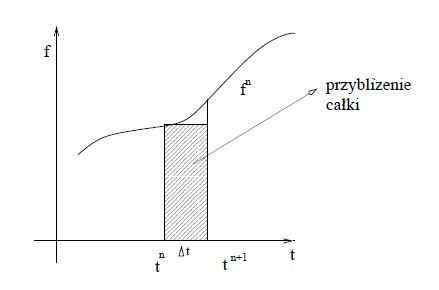
\includegraphics[height=0.65\textheight]{img/22/img1.jpg}
	\end{figure}
\end{frame}
%%%%%%%%%%%%%%%%%%%%%%%%%%
\begin{frame}{Cechy metody}
  \textbf{Algorytm:}
  $$u^{n+1} = u^n - f(u^n, t^n) \cdot \Delta t$$
  \textbf{Cechy:}
  \begin{itemize}
    \item jawna
    \item dokładna jedynie do wyrazów 1-go rzędu ze względu na $\Delta t$ \quad $(\varepsilon=0(\Delta t)$)
    \item prosta
    \item efektywna
  \end{itemize}
\end{frame}
%%%%%%%%%%%%%%%%%%%%%%%%%%
\begin{frame}{Stabilność}
  $t^n$ \quad $u^n, \varepsilon^n$ - błąd \qquad
  $t^{n+1}$ \quad $u^{n+1}, \varepsilon^{n+1}$ 
  \fbox{$\varepsilon^{n+1} = g \cdot \varepsilon^n$\qquad
  g - współczynnik wzmocnienia błędu}

  $$u^{n+1} + \varepsilon^{n+1} = u^n+\varepsilon^n-f(u^n+\varepsilon^n,t^n)\cdot \Delta t \qquad(*)$$
  \underline{zał.:} $\varepsilon^n$ - mały $\Rightarrow$ linearyzacja r. nieliniowego
  $$f(u^n+\varepsilon^n,t^n) = f(u^n,t^n)+\frac{\partial f}{\partial u}{\bigg\arrowvert}_{u^n} \cdot \varepsilon^n+0(\varepsilon^n)$$
  Po podst. do (*):\qquad $\varepsilon^{n+1} = \varepsilon^n-\frac{\partial f}{\partial u}\big\arrowvert_n \cdot \Delta t \cdot \varepsilon^n +0(\varepsilon^n)$ \newline
  \underline{współczynnik wzmocnienia}:\qquad $g = 1- \frac{\partial f}{\partial u}{\big\arrowvert}_n \cdot \Delta t\downarrow$
  warunek stabilności: $|g|<1$ warunek stabilności dla $\frac{\partial f}{\partial u}>0$
  $$\frac{\partial f}{\partial u}\arrowvert_n \cdot \Delta t \leqslant 2 \quad 
  \rightarrow \quad \Delta t \leqslant \frac{2}{\frac{\partial f}{\partial u}\arrowvert_n} \Rightarrow krok$$
  (gdy $\frac{\partial f}{\partial u}\arrowvert_n 0$ - metoda niestabilna)
\end{frame}
%%%%%%%%%%%%%%%%%%%%%%%%%%

\begin{frame}{Przykład}
	\begin{center}
	$\frac{du}{dt}+\frac{u}{\tau} = 0$, \quad $u(0) = 1$\newline $R$, $L\rightarrow \tau = \frac{L}{R}$\qquad rozpad prom.\par
      \begin{itemize}
    \item analitycznie: $u = e^{-\frac{t}{\tau}}$
    \end{itemize}
	\end{center}
  
  krok czasowy gwarantujący stabilność:
  $$\frac{\partial f}{\partial u}\bigg\arrowvert_n = \frac{1}{\tau}\qquad \Delta t \leqslant 2\tau$$
  $\Rightarrow$ \underline{stabilność} - fundamentalna własność metody różnicowej
\end{frame}
%%%%%%%%%%%%%%%%%%%%%%%%%%

\begin{frame}{Przykład 2 - równanie typu oscylacyjnego}
	\begin{center}
		oscylator harmoniczny: \qquad $\frac{d^2x}{dt^2}+ \omega^2x=0$
	\end{center}
    $\Rightarrow$ układ 2 równań:
    $$\left\{\begin{array}{lccll}
	\frac{dx}{dt}&-&\omega^2x&=&0\\
	\frac{dx}{dt}&+&\omega v&=&0\\
	\end{array} \right.$$
    wprowadzenie \qquad \underline{$u = x+iv$} $\Rightarrow$ poj. równanie 1-go rzędu:
    $$ \frac{du}{dt} + i\omega u= 0 \qquad \arrowvert \qquad bo: \quad \frac{dx}{dt} + i\frac{dv}{dt}+i\omega v = 0$$
    \underline{współczynnik wzmocnienia:}
    $$g = 1-{\frac{\partial f}{\partial u}}\bigg\arrowvert _n \cdot \Delta t \quad \Rightarrow \quad g=1-i\cdot \omega \cdot \Delta t \qquad zespolony!$$
\end{frame}
%%%%%%%%%%%%%%%%%%%%%%%%%%

\begin{frame}{Przykład 2 c.d.}
	$$|g|^2 = g \cdot g^* = 1+\omega^2 {\Delta t}^2 \quad \rightarrow \quad 1+\bigg(\frac{\partial f}{\partial u}\bigg{\arrowvert}_n \cdot \Delta t\bigg)^2 > 1 \Rightarrow |g| > 1 $$
    \begin{block}{Uwaga}
    	Metoda Eulera jest bezwzględnie niestabilna dla równań typu oscylacyjnego.
    \end{block}
    W zagadnieniach \textit{nieliniowych $\frac{\partial f}{\partial u}$} jest funkcją $u$ \quad $\Rightarrow$ \quad należy na każdym etapie wybierać $\Delta t$ spełniające warunki stabilności. 
\end{frame}
%%%%%%%%%%%%%%%%%%%%%%%%%%

	\section{Metoda skokowa}
%%%%%%%%%%%%%%%%%%%%%
\begin{frame}{Metoda skokowa}
	\begin{block}{Założenia}
	\begin{itemize}
	\item pochodną względem czasu określamy na podwójnym kroku
    \item kroku pośredniego używamy dla określenia całki
    \item metoda wycentrowana w czasie $\rightarrow $ dokładność drugiego rzędu $\varepsilon = 0({\Delta t}^2)$
	\end{itemize}
	\end{block}
\end{frame}
%%%%%%%%%%%%%%%%%%%%%
\begin{frame}{Algorytm}
	\begin{figure}
	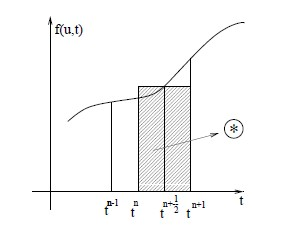
\includegraphics[height=0.5\textheight]{img/22/metoda_skokowa.jpg}
	\end{figure}
    \textbf{Algorytm:}
    $$ \begin{array}{rcl}
      (n+1):\quad &=&u^{n-1} -f(u^n,t^n)\cdot 2 \cdot \Delta t\\
      (n+2):\quad &=&u^n \quad -f(u^{n+1},t^{n+1})\cdot 2 \cdot \Delta t
      \end{array} $$
    
\end{frame}
%%%%%%%%%%%%%%%%%%%%%

\begin{frame}{Trudności}
	\begin{enumerate}
      \item znamy $u^0 = u(0)$, potrzebne $u^1 = u(\Delta t)$; od $u^1$ zależy całkowita dokładność
          \begin{itemize}
            \item podprzedziały w pierwszym $\Delta t$, metoda Eulera,
            \item rozwinięcie w szereg wyższych potęg,
          \end{itemize}
      \item zagadnienie nieliniowe $\Rightarrow$ zmienne $\Delta t$ \quad metoda przestaje być wycentrowana w czasie
    \end{enumerate}
\end{frame}
%%%%%%%%%%%%%%%%%%%%%
\begin{frame}{Współczynnik wzmocnienia błędu}
	$$\varepsilon^{n+1} = \varepsilon^{n-1} - \frac{\partial f}{\partial u} \bigg\arrowvert _n \cdot 2 \cdot \Delta t \cdot \varepsilon^n \quad \arrowvert :\varepsilon^{n-1}$$
    $$\alpha = \frac{\partial f}{\partial u}\bigg\arrowvert_n \cdot \Delta t \qquad g = \frac{\varepsilon^{n+1}}{\varepsilon^n} \ldots$$
    $$g^2 = 1- \alpha \cdot 2g \qquad \underline{g = -\alpha \pm \sqrt{\alpha^2+1}}$$
    Dla metod drugiego rzędu zawsze mamy dwa pierwiastki. \newline
    $\alpha$ - rzeczywiste $\Rightarrow$ \quad $|g| > 1$ \quad $\rightarrow$ niestabilna \quad $\alpha = i\beta, \beta \leqslant 1$, rzeczywiste \newline
    $\Rightarrow g = -i\beta\pm\sqrt{1-\beta^2} \qquad |g|^2 = g \cdot g^* = 1 \quad dla \quad \frac{du}{dt}+i\omega u = 0 \rightarrow \quad \beta = \omega\Delta t \leqslant 1 \quad \rightarrow \quad \Delta t \leqslant\frac{1}{\omega}$
\end{frame}
\begin{frame}{Metoda skokowa dla równań rozpadu}
	$$\frac{du}{dt}+\underbrace{\frac{u}{\tau}}_{f(u,t)} = 0$$\par
    $$ \begin{array}{rcl}
      (n+1):\quad &=&u^{n-1} -f(u^n,t^n)\cdot 2 \cdot \Delta t\\
      (n+2):\quad &=&u^n \quad -f(u^{n+1},t^{n+1})\cdot 2 \cdot \Delta t
      \end{array} $$
      $$\left\{\begin{array}{lll}
      \text{siatka parzysta:}& \text{węzły } 2n&\text{zmienna } \eta\\
      \text{siatka nieparzysta:}&\text{węzły } 2n+1& \text{zmienna }\chi
      \end{array}\right\}\text{  słabo związane}$$
      $$\left\{\begin{array}{lcl}
      \eta^{2n} &=& \eta^{2n-1} - \chi^{2n-1} \cdot\frac{2\Delta t}{\tau}\\
      \chi^{2n+1} &=& \chi^{2n-1} - \eta^{2n} \cdot\frac{2\Delta t}{\tau}
    \end{array}\right.$$
\end{frame}
%%%%%%%%%%%%%%%%%%%%%
\begin{frame}
	Te równania różnicowe są równoważne :
    $$\left\{\begin{array}{lcl}
      \frac{d\eta}{dt}+\frac{\chi}{\tau}&=&0\\
      \frac{d\chi}{dt}+\frac{\eta}{\tau}&=&0
    \end{array}\right.$$
    Dodanie i odjęcie powyższych równań $\Rightarrow$ \quad \textbf{stany własne układu}
    $$\left\{\begin{array}{lcl}
      \frac{d}{dt}(\eta+\chi)+\frac{\eta+\chi}{\tau} & = & 0 \quad \Rightarrow \text{składowa, której szukamy }\\
       & & \qquad \text{(spełnia równanie wyjściowe)}\\
      \frac{d}{dt}(\eta-\chi)+\frac{\eta-\chi}{\tau} & = & 0 \quad \Rightarrow \text{składowa numeryczna,} \\
      & & \qquad \text{zależy od dokładności } u^1\\
      & & \qquad \text{nie jest zgodna z równaniem wyjściowym}
    \end{array}\right.$$
\end{frame}
%%%%%%%%%%%%%%%%%%%%%%%%%%v

		\section{Jawna metoda dwustopniowa (ulepszona Eulera)}
%%%%%%%%%%%%%%%%%%%%%
\begin{frame}{Etap wstępny}
	wyliczenie zmiennej $u$ dla pośredniego $t^{n+\frac{1}{2}}$( metoda Eulera)
    $$u^{n+\frac{1}{2}} = u^n - f(u^n,t^n)\frac{\Delta t}{2} \qquad \text{(wzór pomocniczy)}$$
    $$u^{n+1} = u^n - f(u^{n+\frac{1}{2}},t^{n+\frac{1}{2}})\Delta t \qquad \text{(wzór główny)}$$
\end{frame}
%%%%%%%%%%%%%%%%%%%%%
\begin{frame}
	 \begin{figure}
	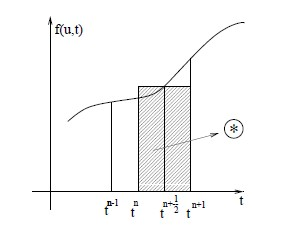
\includegraphics[height=0.6\textheight]{img/22/metoda_skokowa.jpg}
	\end{figure}
\end{frame}
%%%%%%%%%%%%%%%%%%%%%
\begin{frame}{Stabilność}
	$$\varepsilon^{n+1} = \varepsilon^n - \frac{\partial f}{\partial u}\bigg\arrowvert_n\Delta t\bigg[\frac{\partial f}{\partial u} \bigg\arrowvert_n\frac{\Delta t}{2}\bigg]\varepsilon^n$$
    $$g = 1-\alpha +\frac{1}{2}\alpha^2 \qquad \qquad \qquad \alpha = \frac{\partial f}{\partial u}\bigg\arrowvert_n \Delta t$$
    \newline
    - stabilna dla $\alpha$ rzeczywistego, gdy $\Delta t \leqslant \frac{2}{\frac{\partial f}{\partial u}\arrowvert_n}$
    \newline
    - może być niestabilna dla $\alpha$ urojonego
\end{frame}
%%%%%%%%%%%%%%%%%%%%%

	\section{Metoda niejawna drugiego rzędu}
%%%%%%%%%%%%%%%%%%%%%
\begin{frame}{Metoda niejawna drugiego rzędu}
	$$u^{n+1} = u^n - [f(u^n,t^n)+f(u^{n+1},t^{n+1})]\cdot \frac{\Delta t}{2}$$
    \newline
    - $u^{n+1}$ - uwikłane
    \newline
    - metoda ma dokładność 2-go rzędu
\end{frame}
%%%%%%%%%%%%%%%%%%%%%
\begin{frame}{Stabilność}
	$$g = 1-\frac{\partial f}{\partial u}\bigg\arrowvert_n \cdot\frac{\Delta t}{2}-\frac{\partial f}{\partial u}\bigg\arrowvert_{n+1}\cdot \frac{\Delta t}{2} g$$
	$$g=\frac{1-\frac{\partial f}{\partial u}\arrowvert_n \cdot \frac{\Delta t}{2}}{1+\frac{\partial f}{\partial u}\arrowvert_{n+1} \cdot \frac{\Delta t}{2}}$$
    \begin{figure}
    	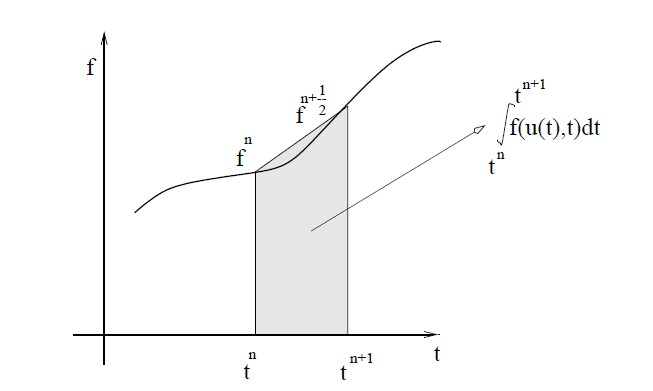
\includegraphics[height=0.55\textheight]{img/22/stabilnosc.jpg}
    \end{figure}
\end{frame}
%%%%%%%%%%%%%%%%%%%%%
\begin{frame}{Stabilność c.d.}
	- równanie rozpadu: $\frac{\partial f}{\partial u} > 0$, \quad $|g| < 1$ (zawsze)
    \newline
    - równanie oscylacyjne $\frac{\partial f}{\partial u}$ - urojone, $|g| = 1$
    \newline\newline
    W obu przypadkach metoda stabilna niezależnie od wyboru kroku
    \begin{itemize}
      \item bezwzględnie stabilna, ważne w zagadnieniach nieliniowych
      \item cena: konieczność rozwiązywania równania algebraicznego na $u^{n+1}$ lub stosowania wzoru iteracyjnego.
    \end{itemize}
\end{frame}
%%%%%%%%%%%%%%%%%%%%%

							\section{Punktowe zagadnienie brzegowe}
%%%%%%%%%%%%%%%%%%%%%
\begin{frame}{Zagadnienie początkowe i brzegowe}
	\begin{tabular}{|l|l|}\hline
	Zagadnienie początkowe & \begin{tabular}{l}
							- ODE spełnia warunki brzegowe\\
    						w jednym punkcie - startowym
							\end{tabular}\\ \hline
    Zagadnienie brzegowe & \begin{tabular}{l}
    					- warunki brzegowe zadane w kilku\\ 
    					 punktach, zwykle na końcach przedziału 
    					\end{tabular} \\ \hline
    \end{tabular}
    \newline\newline
    \begin{block}{Przykładowo:}
    	\begin{itemize}
          \item strzałka ugięcia
          \item przepływ ciepła z T lub $\nabla T$ na brzegach
          \item drgania (membrany)
    	\end{itemize}
    \end{block}
\end{frame}
%%%%%%%%%%%%%%%%%%%%%
\begin{frame}{Przykład}
	\begin{tabular}{|l}
	Szukamy rozwiązania układu H równań różniczkowych zwyczajnych \\
    pierwszego rzędu spełniających $n_1$ warunków brzegowych w punkcie \\
    startu $x_1$ i zbiór pozostałych $n_2 = N-n_1$ warunków brzegowych \\
    w punkcie brzegowym $x_2$.
	\end{tabular}
    $$\frac{dy_i(x)}{dx}= g_i(x, y_1, y_2,\ldots, y_N)\qquad i = 1,2, \ldots, N$$
	w $x = x_1$ rozwiązanie powinno spełniać: \newline
    $$B_{1_j}(x_1, y_1, y_2,\ldots, y_N) = 0\qquad i = 1,2, \ldots, n_1 $$
	w $x = x_2$:
    $$B_{2_k}(x_2, y_1, y_2,\ldots, y_N) = 0 \qquad k = 1,2, \ldots, n_2 $$
\end{frame}
%%%%%%%%%%%%%%%%%%%%%
\begin{frame}
	\begin{block}{Twierdzenie}
		W zagadnieniach fizyki matematycznej:
        $$y'' = f(x,y,y');\qquad y(a) = A, y(b) = B$$
        jeżeli równanie jest \textbf{liniowe:}
        $$y'' = f_1(x)\cdot y'+f_2(x)\cdot y + f_3(X)$$
        to można go \textbf{sprowadzić} do zagadnienia początkowego.
	\end{block}
\end{frame}
%%%%%%%%%%%%%%%%%%%%%
\begin{frame}
	Równanie rozwiązujemy z warunkami początkowymi:
    \begin{center}
    	\begin{tabular}{ccc}
    		$y(a) = A$ & $y'(a)=\alpha_1$ & $y_1(x)$;   $y_1(b) = \beta_1$\\
        	$y(a) = A$ & $y'(a)=\alpha_2$ & $y_2(x)$;   $y_2(b) = \beta_2$
    	\end{tabular}
    \end{center}
    Wtedy funkcja zadana wzorem
    $$y(x) = \frac{1}{\beta_1-\beta_2}[(B-\beta_2)\cdot y_1(x)+(\beta_1-B)\cdot y_2(x)]$$
    spełnia równanie różniczkowe i warunki brzegowe.\newline
    \begin{block}{Rozwiązanie zagadnienia brzegowego}
    	\begin{itemize}
          \item metody strzału (shooting methods)
          \item metody relaksacyjne (relaxation methods)
    	\end{itemize}
    \end{block}
\end{frame}
%%%%%%%%%%%%%%%%%%%%%
\begin{frame}{Metoda strzału}
	\begin{figure}
		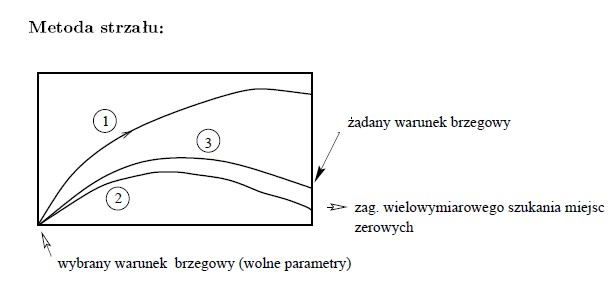
\includegraphics[height=0.55\textheight]{img/5/strzal.jpg}
	\end{figure} 
    Inny wariant:\newline
    \qquad rozpoczęcie całkowania ODE z obu stron, uzgodnienie parametrów przez ,,spotkanie się" rozwiązań w punkcie środkowym.
\end{frame}
%%%%%%%%%%%%%%%%%%%%%
\begin{frame}{Metoda relaksacyjna}
	\begin{figure}
		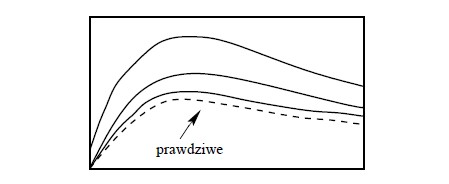
\includegraphics[height=0.35\textheight]{img/5/relaksacyjna.jpg}
	\end{figure}
    \begin{enumerate}
      \item równania różniczkowe $\Rightarrow$ układ równań różniczkowych
      \item iteracyjne poszukiwanie rozwiązań:
          \begin{itemize}
            \item odgadnięte
            \item po pierwszej iteracji
          \end{itemize}
    \end{enumerate}
    \begin{block}{Uwaga!}
    	Rozwiązania próbne nie muszą spełniać ani równania ani warunków brzegowych. 
    \end{block}
\end{frame}
%%%%%%%%%%%%%%%%%%%%%
	\section{Metoda Rungego-Kutty}
%%%%%%%%%%%%%%%%%%%%%
\begin{frame}{Metoda Rungego-Kutty dla pojedynczego równania}
	$$\frac{du(t)}{dt}=f(t,u)\qquad t \in [a,b] \quad u_0 = u(t_0)$$
    Rozwiążanie $u(t)$ wyznaczamy w punktach
    $$t_i = t_0+i\cdot h \qquad h=\frac{b-a}{n}, \quad i = 0,1,\ldots,n$$
    W metodach jednokrokowych jawnych rozwiązanie:
    $$u_{i+1} = u_i + h\cdot F(t_i,u_i,h) \qquad i = 0,1,\ldots,n-1 \qquad(*)$$
    F - zadana funkcja
\end{frame}
%%%%%%%%%%%%%%%%%%%%%
\begin{frame}{Metody R-K - szczególny przypadek (*)}
	$$u(t_{i+1}) = u(t_i)+h\cdot u'(t_1)+\frac{h^2}{2}\cdot u''(t_i)+\ldots+\frac{h^q}{q!}\cdot u^{(q)}(t_i) + R$$
    dla \textbf{i = 0} :
    $$u_1 = u(t_0) + h\cdot \underbrace{u'}_{!!}(t_0)+\frac{h^2}{2}\cdot\underbrace{u''}_{!!}(t_0)+\ldots+\frac{h^q}{q!}\cdot \underbrace{u^{(q)}}_{!!}(t_0) \qquad (**) $$
    \begin{flushright}
    	!! - należy wyznaczyć
    \end{flushright}
    \begin{center}
    	\begin{tabular}{|r|} \hline
    		$u'(t_0)=f(t_0,u_0)$\\ \hline
        	$u''(t_0) = \frac{\partial f}{\partial t}\arrowvert_0+\frac{\partial f}{\partial u}\arrowvert_0 \cdot u'_0 = \frac{\partial f}{\partial t}\arrowvert_0 + \frac{\partial f}{\partial u}\arrowvert_0 \cdot f(t_0,u_0)$\\ \hline
        itd... \\ \hline
       		$u'(t_0)$ - prosto, wyższe - uciążliwe obliczenia!\\ \hline
    	\end{tabular}
    \end{center}
\end{frame}
%%%%%%%%%%%%%%%%%%%%%
\begin{frame}
	Równanie (**) można zapisać jako:
    \begin{tabular}{ccl}
    $u_1$ & = & $u_0+h \cdot \bigg[u'(t_0)\frac{h}{2}u''(t_0) +\ldots+\frac{h^{q-1}}{q!}u^{(q)}(t_0)\bigg] =$\\
     & = & $u_0 + h \cdot \bigg[f(t_0,u_0)+\frac{h}{2}\cdot f^{(1)}(t_0,u_0)+\ldots+\frac{h^{q-1}}{q!}f^{q-1}(t_0,u_0)\bigg]$
    \end{tabular}
    gdzie:
    $$f^{(s)}(t_0,u_0) = \frac{d^s}{dt^s}f(t,u(t))\bigg\arrowvert_{t=t_0, u(t)=u_0} \qquad s = 1,2,\ldots,q-1$$
    \begin{block}{Idea metod Rungego-Kutty}
    Ideą metod jest dobranie funkcji F (wzór *):
    	\begin{itemize}
          \item bez wyznaczania pochodnych $f^{(s)}(t_0,u_0)$
          \item tak, by jak najlepiej przybliżyła funkcję $F_T$
    	\end{itemize}
    \end{block}
\end{frame}
%%%%%%%%%%%%%%%%%%%%%
\begin{frame}{R-punktowa metoda Rungego-Kutty}
	$$(***)\left\{\begin{array}{l}
	u_{i+1} = u_i + h F(t_i,u_i,h), \qquad i = 0,1,2,\ldots,n-1\\
    F(t,u,h) = c_1k_1(t,u,h) + c_2k_2(t,u,h)+\ldots+c_rk_r(t,u,h)\\
    k_1(t,u,h) = f(t,u) \\
    k_j(t,u,h) = f(t+ha_j,u+h \sum_{n=1}^{j-1}b_{js}k_s(t,u,h)), \quad j = 2,\ldots,r \\
    a_j = \sum_{s=1}^{j-1}b_{js}
	\end{array}\right.$$
    $a_j, b_{js}, c_k$ - stałe rzeczywiste, dobrane tak, aby:
    $$\phi(h) = F(t,u,h) - F_T(t,u,h)$$
    zawierała jedynie potęgi $h$ możliwie wysokiego rzędu. 	
\end{frame}
%%%%%%%%%%%%%%%%%%%%%
\begin{frame}
	Niech:
    \begin{tabular}{lcll}
    $\alpha$ & = & $\frac{\partial f}{\partial t}+f\frac{\partial f}{\partial u}$ & \\
    $\beta$ & = & $\frac{\partial^2f}{\partial t^2}+2f\frac{\partial^2f}{\partial t \partial u}+f^2\frac{\partial^2f}{\partial u^2}$ & f = f(t,u)
    \end{tabular}
 	\newline \newline \par
    Dla $r = 0$ wzory (***) mają postać:
   	\newline
    \begin{tabular}{rcl}
    	$F(x,y,h)$ & $=$ & $c_1 \cdot k_1 + c_2 \cdot k_2 + c_3 \cdot k_3$ \\
        $k_1$ & $=$ & $f(t,u)$ \\
        $k_2$ & $=$ & $f(t + h \cdot a_2, u + h \cdot b_{21} \cdot k_1 =$ \\
         & $=$ & $f(t+a_2 \cdot h, u+h \cdot a_2 \cdot k_1) $\\
        $k_3$ & $=$ & $f(t+a_3 \cdot h, u+h \cdot (b_{31} \cdot k_1 + b_{32} \cdot k_2)) = $ \\
         & $=$ & $f(t+a_3 \cdot h, u+h \cdot (a_3 - b_{32}) \cdot k_1 + h \cdot b_{32} \cdot k_2)$
    \end{tabular}
\end{frame}
%%%%%%%%%%%%%%%%%%%%%
\begin{frame}
	$k_2, k_3$ rozwijamy w szereg Taylora wokół (t,u):
    \begin{flushleft}
    	$k_2=f(t,u)+ha_2\bigg(\frac{\partial f}{\partial t}+k_1\frac{\partial f}{\partial u}\bigg) + \frac{1}{2}h^2a_2^2\bigg(\frac{\partial^2f}{\partial t^2}+k_1\frac{\partial^2f}{\partial t \partial u}+k_1^2\frac{\partial^2f}{\partial u^2}\bigg)+O(h^3)$ \newline
        $k_2 = f(t,u)+ha_2\alpha+\frac{1}{2}h^2a_2^2\beta+O(h^3)$ \newline
        $k_3 = f(t,u)+ha_3\alpha + h^2(a_2 \cdot b_{32} \cdot \alpha \frac{\partial f}{\partial u} + \frac{1}{2}a_3^2\beta) + O(h^3)$
    \end{flushleft}
    stąd:
    \begin{tabular}{r}
    	$\varphi(h) = F(t,u,h) - F_T(t,u,h) = $\\
    	$ = (c_1+c_2+c_3-1) \cdot f(t,u)+h \cdot \alpha \cdot (c_2 \cdot \alpha^2 + c_3 \cdot a_3 - \frac{1}{2}) + $ \\
        $+ h^2 \cdot \big[c_3a_3b_{32}\alpha\frac{\partial f}{\partial u}+\frac{1}{2}(c_2 \cdot a_2^2 +c_3a_3^2)-\frac{1}{6}(\alpha \cdot \frac{\partial f}{\partial u}+\beta)\big]+O(h^3) $
    \end{tabular}
    \begin{block}{Uwaga!}
    	Należy dobrać $c_1, c_2, c_3, a_2, a_3, b_{32}$ w taki sposób, aby w $\varphi(h)$ były tylko potęgi możliwie wysokiego stopnia.
    \end{block}
\end{frame}
%%%%%%%%%%%%%%%%%%%%%
\begin{frame}
	\fbox{\textbf{r = 1}}
    $$c_2=c_3=a_2=a_3=b_{32}=0$$
    Przyjmuje się $c_1 = 1$ \qquad $\Rightarrow \left.\begin{array}{l}
    \varphi(h) = O(h) \\
    f(t,u,h) = f(t,u)
    \end{array}\right.$
    $$u_{i+1} = u_i + h \cdot f(t_i,u_i), \qquad i = 0,1, \ldots,n-1$$
    \begin{block}{Wniosek}
    	Jest to metoda Eulera.
    \end{block}
\end{frame}
%%%%%%%%%%%%%%%%%%%%%
\begin{frame}
	\fbox{\textbf{r = 2}}
    $$c_3 = b_{32} = 0$$
    $\left\{\begin{array}{rcl}
    	c_1 + c_2 - 1 & = & 0\\
        c_2 \cdot a_2 - \frac{1}{2} & = & 0
    \end{array}\right. \qquad\Rightarrow \qquad \varphi(h) = O(h^2)$
    \begin{enumerate}
      \item $c_1 = 0, c_2 = 1, a_2 = \frac{1}{2} \quad \Rightarrow \quad F(t,u,h) = f(t+\frac{1}{2}h, u+\frac{1}{2}h \cdot f(t,u)) \rightarrow \text{zmodyfikowana metoda Eulera}$
      \item $c_1 = \frac{1}{2}, c_2 = \frac{1}{2}, a_2 = 1 \quad\Rightarrow\quad F(t,u,h) = \frac{1}{2} \cdot[f(t,u)+f(t+h,u+h \cdot f(t,u))]$
    \end{enumerate}
\end{frame}
%%%%%%%%%%%%%%%%%%%%%
\begin{frame}
	\fbox{\textbf{r = 3}}
    \begin{center}
    	Dobieramy $c_1,c_2,c_3,a_2,a_3,b_{32}$, tak, aby w $\varphi(h)$ współczynniki przy $h^0,h,h^3$ - były zerowe:
        $$\left\{\begin{array}{l}
        c_1+c_2+c_3 = 1\\
        c_2a_2+c_3a_3 = \frac{1}{2} \\
        c_3a_2^2+c_3a_3^2 = \frac{1}{3} \\
        c_3a_2b_{32} = \frac{1}{6}
        \end{array}\right.\rightarrow\left.\begin{array}{c}
        \text{4 równania, 6 niewiadomych}\\
        \Rightarrow \\
        \text{Trójpunktowa metoda Rungego-Kutty} \\
        c_1 = \frac{1}{6},\quad c_2 = \frac{2}{3}, \quad c_3 = \frac{1}{6} \\
        a_2 = \frac{1}{2},\quad a_3 = 1, \quad b_{32} = 2
        \end{array}\right.$$
    \end{center}
\end{frame}
%%%%%%%%%%%%%%%%%%%%%
\begin{frame}{Praktyczne znaczenie - 4-punktowe wersje metody Rungego-Kutty}
	a)
    \begin{center}
    	\begin{tabular}{l}
    		$u_{i+1} = u_i+\frac{h}{6}(k_1+2k_2+2k_3+k_4)$, $\qquad i = 0,1,2, \ldots,n-1$\\
            $k_1 = f(t_i,u_i)$,\\
            $k_2 = f(t_i+\frac{1}{2}h,u_i+\frac{1}{2}hk_1)$,\\
            $k_3 = f(t_i+\frac{1}{2}h,u_i+\frac{1}{2}hk_2)$,\\
            $k_4 = f(t_i+h,u_i+hk_3)$
    	\end{tabular}
    \end{center}
    b) 
      \begin{center}
    	\begin{tabular}{l}
    		$u_{i+1} = u_i+\frac{h}{8}(k_1+3k_2+3k_3+k_4)$, $\qquad i = 0,1,2, \ldots,n-1$\\
            $k_1 = f(t_i,u_i)$,\\
            $k_2 = f(t_i+\frac{1}{3}h,u_i+\frac{1}{3}hk_1)$,\\
            $k_3 = f(t_i+\frac{2}{3}h,u_i-\frac{1}{3}hk_1+hk_2)$,\\
            $k_4 = f(t_i+h,u_i+hk_1-hk_2+hk_3)$
    	\end{tabular}
    \end{center}
  	Dla obu: $\varphi_4(h) = O(h^5)$
\end{frame}
%%%%%%%%%%%%%%%%%%%%%
\begin{frame}{Wada metod R-4}
	\textbf{Wada:} \quad np. dla \textbf{r = 4}, na etapie 1 kroku obliczeń wartość $f$ jest wyznaczana 4 razy i nie będą to wartości użyteczne na dalszych etapach.\newline\par
    \begin{itemize}
      \item Ćwiczenia z metod Rungego-Kutty
      \item Procedura w Fortranie dla metody R-4
      \item Metoda Rungego-Kutty dla programu Mathematica
    \end{itemize}
\end{frame}
%%%%%%%%%%%%%%%%%%%%%
	\section{Metody Rungego-Kutty dla układów ODE}
%%%%%%%%%%%%%%%%%%%%%
\begin{frame}{Metody R-K dla układów ODE}
	$$\left\{\begin{array}{l}
		\vec{u}(t) = (u_1(t),u_2(t),\ldots,u_m(t))\\
        \vec{f}(t,\vec{u}) = (f_1(t,\vec{u}),f_2(t,\vec{u}),\ldots,f_m(t,\vec{u}))\\
        \vec{u_0}
	\end{array}\right.$$
    układ równań:
    $$\left\{\begin{array}{l}
    	\frac{d}{dt}\vec{u}(t) = \vec{f}(t,\vec{u}(t)), \qquad t\in[a,b]\\
        \text{z warunkiem początkowym } \vec{u}(t_0) = \vec{u}_0
    \end{array}\right.$$
\end{frame}
%%%%%%%%%%%%%%%%%%%%%
\begin{frame}{Postać r-punktowej metody R-K}
	$$\vec{u}_{i+1} = \vec{u}_i + h \cdot \vec{F}(t_i,\vec{u}_i,h)$$
    gdzie:
    \begin{tabular}{lcl}
    	$\vec{F}(t,\vec{u},h)$ & = & $c_1 \cdot k_1(t,\vec{u},h)+c_2 \cdot k_2(t_1,\vec{u},h)+\ldots+c_rk_r(t,\vec{u},h)$ \\
        $\vec{k}_1(t,\vec{u}, h)$ & = & $f(t,\vec{u})$,\\
        $\vec{k}_j(t,\vec{u},h)$ & = & $\vec{f}(t+h \cdot a_{j_1}\vec{u} + h \cdot \sum_{s = 1}^{j-1}b_{js}\vec{k}_s(t,\vec{u},h))$, $j = 2,3,\ldots,r$
    \end{tabular}
    $$a_j = \sum_{s = 1}^{j-1}b_{js}, \qquad j = 2,3,\ldots,r$$
    $a_j,b_{js},c_r$ - stałe rzeczywiste, wartości takie same jak dla pojedynczego równania.
\end{frame}
%%%%%%%%%%%%%%%%%%%%%

    
\end{document}
